As we mentioned, GDSDA is a paradigm using generalized distillation for domain adaptation. In this section, we first give a brief review of generalized distillation. Then we show the process of GDSDA and demonstrate the reason why GDSDA can work with the SDA problem. Finally, we show that to achieve an optimal model, we should carefully set the value of imitation parameter to minimize the training error. 
\begin{figure}
\centering
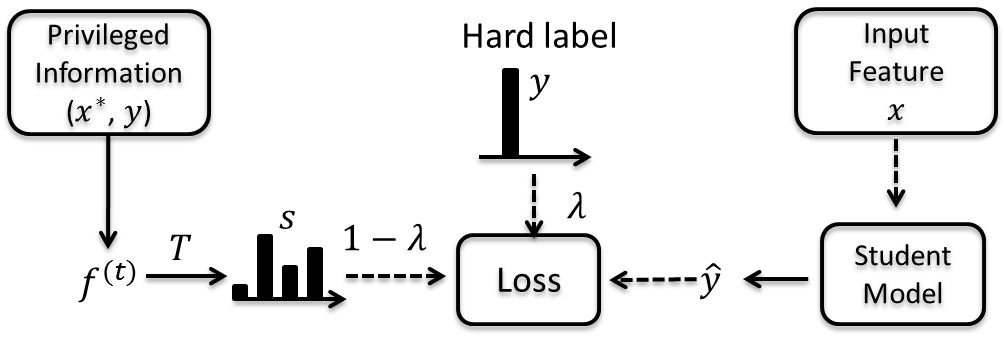
\includegraphics[scale=.4]{figure/GD.png}
\caption{Illustration of Generalized Distillation training process.}
\end{figure}
\subsection{An overview of Generalized Distillation and GDSDA}
\textit{Distillation} \cite{hinton2015distilling} and \textit{Learning Using Privileged Information} (LUPI) \cite{vapnik2015learning} are two paradigms that enable machines to learn from other machines. Both methods address the problem how to build a student model that can learn from the advanced teacher models. Recently, Lopez {et al.} \cite{lopez2015unifying} proposed a framework called \textit{generalized distillation} that unifies both techniques and show that it can be applied in many scenarios.

In GD, the training data can be represented as a collection of the triples:
\[\{\left(x_1,x_1^*,y_1\right),\left(x_2,x_2^*,y_2\right) \dots \left(x_n,x_n^*,y_n\right)\}\]
where $x^*$ is the privileged information associate to the label $y$ which is not accessible in the test process. Therefore, the goal of GD is to train a model, called student model with the guidance of the the privileged information.

The process of generalized distillation is as follows: in step 1, a teacher model ${f}^{(t)}$ is trained using the input-output pairs $\{x^*_i,y_i\}_{i=1}^n$. In step 2, use ${f}^{(t)}$ to generate the soft label $s_i$ for each training example $x_i$ using with the softmax function $\sigma$:
\begin{equation}\label{eq:softmax_T}
s_i=\sigma(f^{(t)}(x_i)/T)
\end{equation}
where $T$ is a parameter called temperature to control the smoothness of the soft label. In step 3, learn the student ${f}^{(s)}$ using the pair $\{\left(x_i,y_i\right),\left(x_i,s_i\right)\}_{i=1}^n$ using:
\begin{equation}\label{eq:distill}
\begin{aligned}
f^{(s)}=&\underset{f^{(s)} \in \mathcal{F}^{(s)}}{\arg \min}\frac{1}{n}\sum_{i=1}^{n}[\lambda\ell\left(y_i,\sigma(f^{(s)}(x_i))\right)\\
&+(1-\lambda)\ell\left(s_i,\sigma(f^{(s)}(x_i))\right)]\\
\end{aligned}
\end{equation}
Here, $\lambda$ is the imitation parameter to balance the importance between the hard label $y_i$ and the soft label $s_i$.

